\documentclass[12pt]{article}
\usepackage{preamble}

\pagestyle{fancy}
\fancyhead[LO,LE]{Физические основы компьютерных \\ и сетевых технологий}
\fancyhead[CO,CE]{14.10.2024}
\fancyhead[RO,RE]{Лекции Музыченко Я. Б.}

\fancyfoot[L]{\scriptsize исходники найдутся тут: \\ \url{https://github.com/pelmesh619/itmo_conspects} \Cat}

\begin{document}
    \section{6. Гироскоп. Механическая работа.}

    Повторим то, что было на прошлой лекции. Рассмотрим два типа движения:

    \mediumvspace

    \begin{multicols}{2}
        \begin{tcolorbox}[title=Поступательное движение]
            $d\vec{r}; x, y, z$

            $\vec{v} = \frac{d\vec{r}}{dt}$

            $\vec{a}_\tau = \frac{d\vec{v}}{dt}$

            $m$

            $\vec{p} = m\vec{v}$

            $\vec{p} = const$ при $\vec{F}_\text{вн.} = 0$ (ЗСИ)

            $\vec{F} = m\vec{a}$

            $\vec{F} = \frac{d\vec{p}}{dt}$
        \end{tcolorbox}
        
        \begin{tcolorbox}[title=Вращательное движение]
            $d\vec{\varphi}$

            $\vec{\omega} = \frac{d\vec{\varphi}}{dt}$

            $\vec{\beta} = \frac{d\vec{\omega}}{dt}$

            $I \qquad I_{\text{м.т.}} = mr^2, \hfill I = \int r^2 dm$

            $\vec{L} = I \vec{\omega} \hfill \vec{L} = [\vec{r}\vec{p}]$

            $\vec{L} = const$ при $\vec{M}_\text{вн} = 0$ (ЗСМИ)

            $M_z = I\beta_z$

            $\vec{M} = \frac{d\vec{L}}{dt} \hfil = [\vec{r}\vec{F}]$
        \end{tcolorbox}
    \end{multicols}

    \smallvspace
    
    \begin{minipage}{\textwidth}
        \begin{wrapfigure}{r}{0pt}
            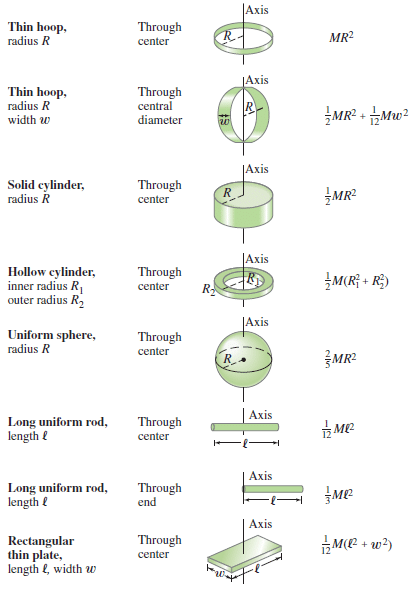
\includegraphics[width=6cm]{physics1/images/physics1_2024_10_14_1}
        \end{wrapfigure}

        Теорема Штейнера: момент инерции $I$ тела относительно произвольной неподвижной оси равен сумме момента инерции этого тела 
        $I_0$ относительно параллельной ей оси, проходящей через центр масс тела, и произведения массы тела $m$ на квадрат расстояния 
        $d$ между осями:

        \[I = I_0 + md^2\]

        Также мы рассмотрели моменты инерции для разных тел

        \subsection{Гироскоп}

        Рассмотрим вращающийся волчок: вращаясь, он постепенно теряет энергию из-за трения и сопротивления воздуха, из-за чего
        его вращение замедляется, и его ось начинает вращаться по другой оси. 
    \end{minipage}
        
    \begin{minipage}{\textwidth}
        \begin{wrapfigure}{r}{0pt}
            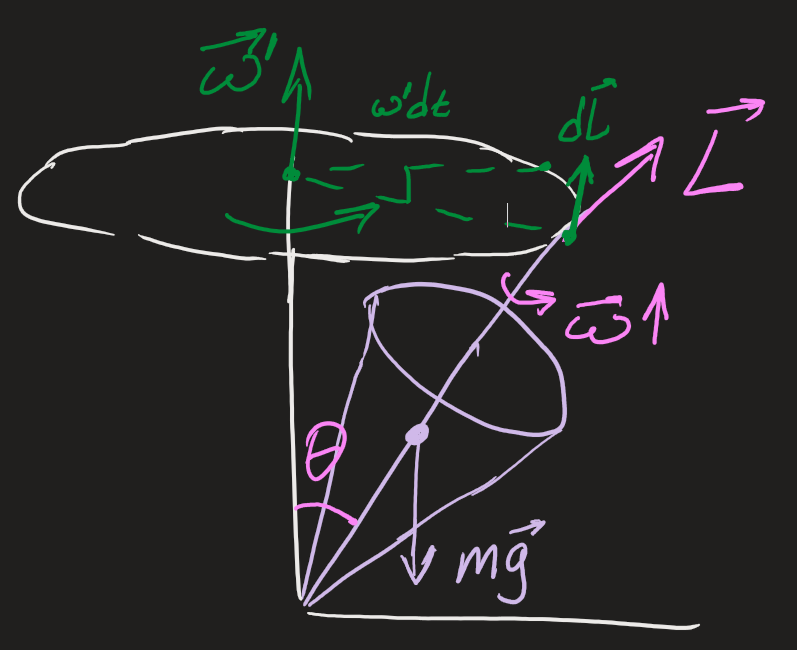
\includegraphics[width=6cm]{physics1/images/physics1_2024_10_14_2}
        \end{wrapfigure}
        
        Обозначим за $\vec{L}_\omega$ момент инерции 
        волчка и за $\vec{L}^\prime$ момент инерции оси. Тогда:
        
        $\vec{L} = \vec{L}_\omega + \vec{L}^\prime$

        $\vec{L}_\omega = I \vec{\omega}$

        Заметим, что в опыте скорость вращения волчка намного больше скорости вращения оси $\omega \gg \omega^\prime$

        Из этого $d\vec{L} = L \sin\theta \cdot \omega^\prime dt$

    \end{minipage}
    
    \smallvspace

    Или в векторной форме:

    $d\vec{L} = [\vec{\omega}\vec{L}]dt$

    $\vec{M} = [\vec{\omega}\vec{L}]$

    Также заметим, что $L_\omega \gg L^\prime$

    Способность сохранять положение вращающегося волчка используется в таком приборе, как гироскоп. 
    Гироскоп применяется для определения положения аппарата (например, самолет, космического корабля) в авионике.



    \subsection{Механическая работа}

    $d\vec{r}$ - элементарное перемещение, в пределах которого сила $\vec{F}$ постоянна

    $Fs$ - проекция силы на направление перемещения

    $d\vec{r} = ds$

    Элементарная работа силы $\vec{F}$ на перемещении $d\vec{r}$

    $dA = \vec{F} d\vec{r} = F\cdot ds \cos \alpha = F_s ds$

    $A = \sum dA = \int dA$

    $A = \int_1^2 \vec{F}d\vec{r} = \int_1^2 F_s ds$

    Допустим на тело действует несколько сил:

    $\vec{F} = \vec{F}_1 + \vec{F}_2 + \dots$

    $A = \int_1^2 \vec{F}d\vec{r} = \int_1^2 (\vec{F}_1 + \vec{F}_2 + \dots) d\vec{r}$

    Мощность - скалярная величина, равная работе силы, совершаемой за единицу времени. Характеризует скорость, с которой совершается работа

    $N = \frac{dA}{dt} = \frac{\vec{F}d\vec{r}}{dt} = \vec{F}\vec{v}$

    $A = \int Ndt$

    Работа силы упругости: $A = \int_{x_1}^{x_2} (-kx)dx = \frac{kx^2_1}{2} - \frac{kx_2^2}{2}$

    Работа силы тяжести: $A = \int_1^2 m\vec{g}d\vec{r} = mgh_1 - mgh_2$

    Работа силы тяготения: $A = \int_{r_1}^{r_2} \frac{Gm_1 m_2}{r^2} dr = - \frac{Gm_1 m_2}{r} \Big|_{r_1}^{r_2} = \frac{Gm_1 m_2}{r_1} - \frac{Gm_1 m_2}{r_2}$

    Силы, чья работа не зависит от траектории пути, будет называть \textit{консервативными} (потенциальными)

    Тогда из этого мы можем вывести потенциальную энергию:

    Потенциальная энергия для силы упругости: $U = \frac{kx^2}{2}$

    Потенциальная энергия для силы тяжести: $U = mgh$

    Потенциальная энергия для силы тяготения: $U = \frac{Gm_1 m_2}{r}$

    В общем виде получаем $A = U_1 - U_2$

    $dA = -dU \qquad \vec{F}d\vec{r} = -dU$

    $\vec{F} = -(\frac{\partial u}{\partial x}\vec{i} + \frac{\partial u}{\partial y}\vec{j} + \frac{\partial u}{\partial z}\vec{k})$

    $\vec{F} = -\mathrm{grad}\, U = -\nabla U$
\end{document}

